\subsection{25. Анализатор перенос-свёртка, недостатки анализатора.}
\textbf{Мотивировка:} У нас есть алгоритм Эрли, но он работает долго.
\begin{itemize}
    \item Scan: $O(|w|^2|G|)$
 \item Predict: $O(|w|^2|G|^2)$
\item  Complete:$O(|w|^3|G|^2)$
\end{itemize}
Чтобы понять алгоритм, \textbf{рассмотрим грамматику и слово w = ab}\\
\begin{itemize}
    \item $S' \rightarrow S$(добавляем)
 \item $S \rightarrow aB$
 \item $B \rightarrow b$
\end{itemize}
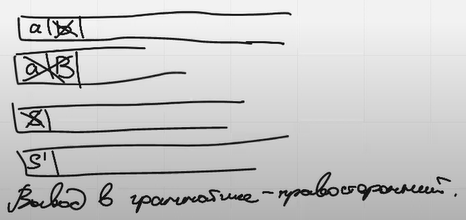
\includegraphics[width=7cm]{form1.PNG}\\
\begin{itemize}
    \item[] Храним стек текущих символов и текущую позицию в слове.

 \item На вершине стека написана правая часть правила - заменяем на левую (reduce)

 \item Иначе - добавляем символ в стек и читаем символ (shift)
\end{itemize} Стоит заметить, что разбираем мы слово справа налево, а вывод в грамматике правсторонний, поэтому мы будем вынуждены поменять порядок правил на обратный для построения дерева разбора
\\
\textbf{А в чем проблема?}
\begin{itemize}
    \item [1] А как понять, какая правая часть правила находится на стеке?
     \item [2] А что делать, если нам подходят несколько правил? (стек можно распарсить двумя и более способами) 
\end{itemize}